% !TeX root = RJwrapper.tex
\title{Editorial}


\author{by Emi Tanaka}

\maketitle


\section*{In this issue}\label{in-this-issue}
\addcontentsline{toc}{section}{In this issue}

On behalf of the editorial board, I am pleased to present Volume 18 Issue 2 of the R Journal. This issue features fifteen research articles, plus news from the R Foundation, Forwards Taskforce, Bioconductor and changes from CRAN.

This issue highlights the continued growth and diversity of the R ecosystem, bringing together contributions that advance statistical methodology, computational tools, and domain-specific applications. New packages introduce methods for Bayesian inference for complex spatial point processes (\CRANpkg{binspp}) and spatial boundary analysis (\CRANpkg{nimblewomble}), nonparametric autocovariance estimation (\CRANpkg{CovEsts}), data-driven trend and seasonality estimation (\CRANpkg{deseats}), space-filling designs for computer experiments (\CRANpkg{SFDesign}), and functional-data-based insurance reserving (\CRANpkg{ProfileLadder}). Developments in modern machine learning and uncertainty quantification are represented by \CRANpkg{DeepLearningCausal}, which combines deep neural networks, ensemble learning, and conformal prediction for causal inference, alongside a review of conformal prediction tools available in R. The issue also features software for transparent evidence synthesis in network meta-analysis (\CRANpkg{NMAforest}), educational test data engineering (\CRANpkg{exametrika}), precision agriculture using multispectral imagery (\CRANpkg{rPAex}), scalable record linkage (\CRANpkg{blocking}), and text comparison and visualisation (\CRANpkg{highlightr}). Complementing these methodological advances are improvements to data visualisation through \CRANpkg{woylier}, which introduces a new interpolation approach for high-dimensional tours, and software interoperability through \CRANpkg{kerasnip}, which bridges \CRANpkg{keras3} and the \CRANpkg{tidymodels} ecosystem. Collectively, these articles demonstrate the continued strength of the R community in developing accessible, extensible, and practically useful software that supports modern statistical analysis across a wide range of disciplines.

All packages discussed are available on CRAN. Supplementary material with fully reproducible code is available for download from the R Journal website.

\section*{2026 Rousseeuw Prize for Statistics Awarded to the R Core Team}\label{rousseeuw-prize-for-statistics-awarded-to-the-r-core-team}
\addcontentsline{toc}{section}{2026 Rousseeuw Prize for Statistics Awarded to the R Core Team}

The Rousseeuw Prize, named after statistician Peter Rousseeuw, recognises major contributions that have transformed the practice of statistics and its impact on society. The 2026 Rousseeuw Prize for Statistics has been awarded to five members of the R Core Team in recognition of their decades-long work developing and maintaining R, the open-source statistical computing language that has become foundational to modern data science.

The 2026 prize recipients are \textbf{Brian D. Ripley} (University of Oxford), \textbf{Martin Maechler} (ETH Zurich), \textbf{Kurt Hornik} (WU Vienna University of Economics and Business), \textbf{Peter Dalgaard} (Copenhagen Business School), and \textbf{Luke Tierney} (University of Iowa). They are recognised for their sustained contributions to the R project; half of the prize is awarded to these five individuals, with the remaining half shared among other members of the R Core Team in acknowledgement of the collective nature of the work.

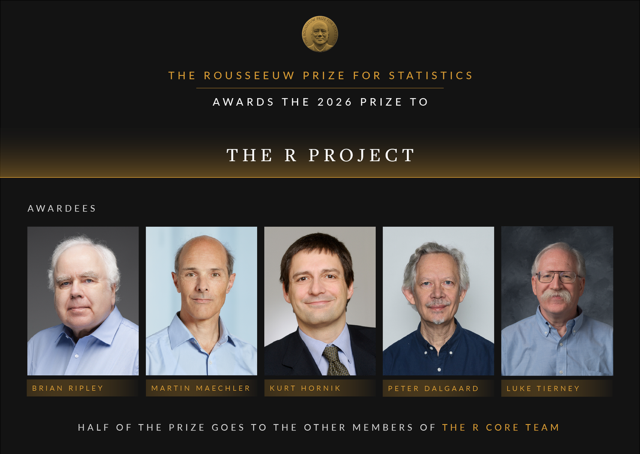
\includegraphics[width=1\linewidth]{Rousseeuw Prize - Laureates 2026}

Over nearly three decades, the R Core Team and contributors have built R into a global infrastructure for statistical computing, enabling reproducible research and lowering barriers to advanced analytics. Today, R underpins thousands of research projects and educational programs worldwide and is widely used by organisations including regulatory agencies, pharmaceutical companies, and central banks. Congratulations to the R Core Team on this well-deserved recognition!


\address{%
Emi Tanaka\\
Australian National University\\%
\\
%
\url{https://journal.r-project.org}\\%
%
\href{mailto:r-journal@r-project.org}{\nolinkurl{r-journal@r-project.org}}%
}
